
\section{Shell Preliminaries}

As our work extends and use~\cite{jiang2020bijective}, we briefly overview the main definition and notation therein. %We refer to their paper for a complete description and for the algorithm to construct it.
\cite{jiang2020bijective} introduces an algorithm to construct a shell around a given triangle mesh. 

\paragraph{Shell.} The shell is defined by three triangle surface meshes $\PS = \{(B_s,V_s,T_s),F_s\}$ sharing the same mesh connectivity $F_s$, where $B_s, V_s,$ and $T_s$ are the vertices of the bottom, middle, and top surface respectively. Every triangle in $F_s$ corresponds to a generalized prism, defined connecting the corresponding triangle in the three surfaces with straight edges, called \emph{pillars}. Every prism $P$ has three vertices $v_i\in V_s, t_i\in T_s, b_i\in B_s, i=1,2,3$ on the middle, top, and bottom surface, respectively. Each pillar decomposes into a top $h_i^T = t_i - v_i, i=1,2,3$ and bottom $h_i^B = b_i - v_i, i=1,2,3$ part, and each part can be canonically decomposed into 3 tetrahedra, and each tetrahedra is assigned with a constant vector field aligned with the pillars it is connected with ~\cite[Figure 5]{jiang2020bijective}, which is used to define a projection operator $\Pi$ within the shell. 

\paragraph{Projection Operator.} For every prism $P$, the projection operator $\Pi_P$ is defined as the piecewise constant vector field $V$ inside the decomposed prism, by assigning to each tetrahedron $T^P_j, j = 1, \dots, 6$, the constant vector field defined by the only edge of $T^P_j$ which one of the oriented pillars $h_i^T, h_i^B, i=1,2,3$. That is, $\forall p \in T^P_j$
\[
\Pi_P(p)=h_i^K, 
\]
where $i$ is the index of the vertex corresponding to the pillar edge of $T^P_j$ and $K$ is either the top or bottom surface. The shell projection operator $\Pi$ is defined as the \TS{union} of all local projections $\Pi_P$.

\paragraph{Section.} A triangle mesh  is a section if it is contained within the shell, and if the dot product of the normal of each of its triangles with the vector field in the overlapping tetrahedra is positive. The projection operator $\Pi$ defines a bijective map between any pair of sections if the shell is valid.

\paragraph{Shell Validity.}
\cite{jiang2020bijective} defines a shell $\PS$ to be \emph{valid} with respect to an input mesh $\M$ if it satisfies two invariants:
\begin{enumerate}
    \item The volumes of all possible tetrahedral decomposition of a prism (24 of them) are positive.
    \item $\M$ is a section for all possible tetrahedral decomposition. That is, the input mesh is contained within the shell, and the dot product between the mesh's normals and the shell's pillar is positive. 
\end{enumerate}

\DP{Figure for shell and projection}

The algorithm to build the shell creates an initial valid shell, potentially thin and dense, and then uses local operations to improve its quality while preserving the validity \cite{jiang2020bijective}.

\DP{No intro to curved meshing? I though it was a good idea. Otherwise we need to be more precise when we describe the output.}

\section{Method}

\begin{figure}
    \centering
    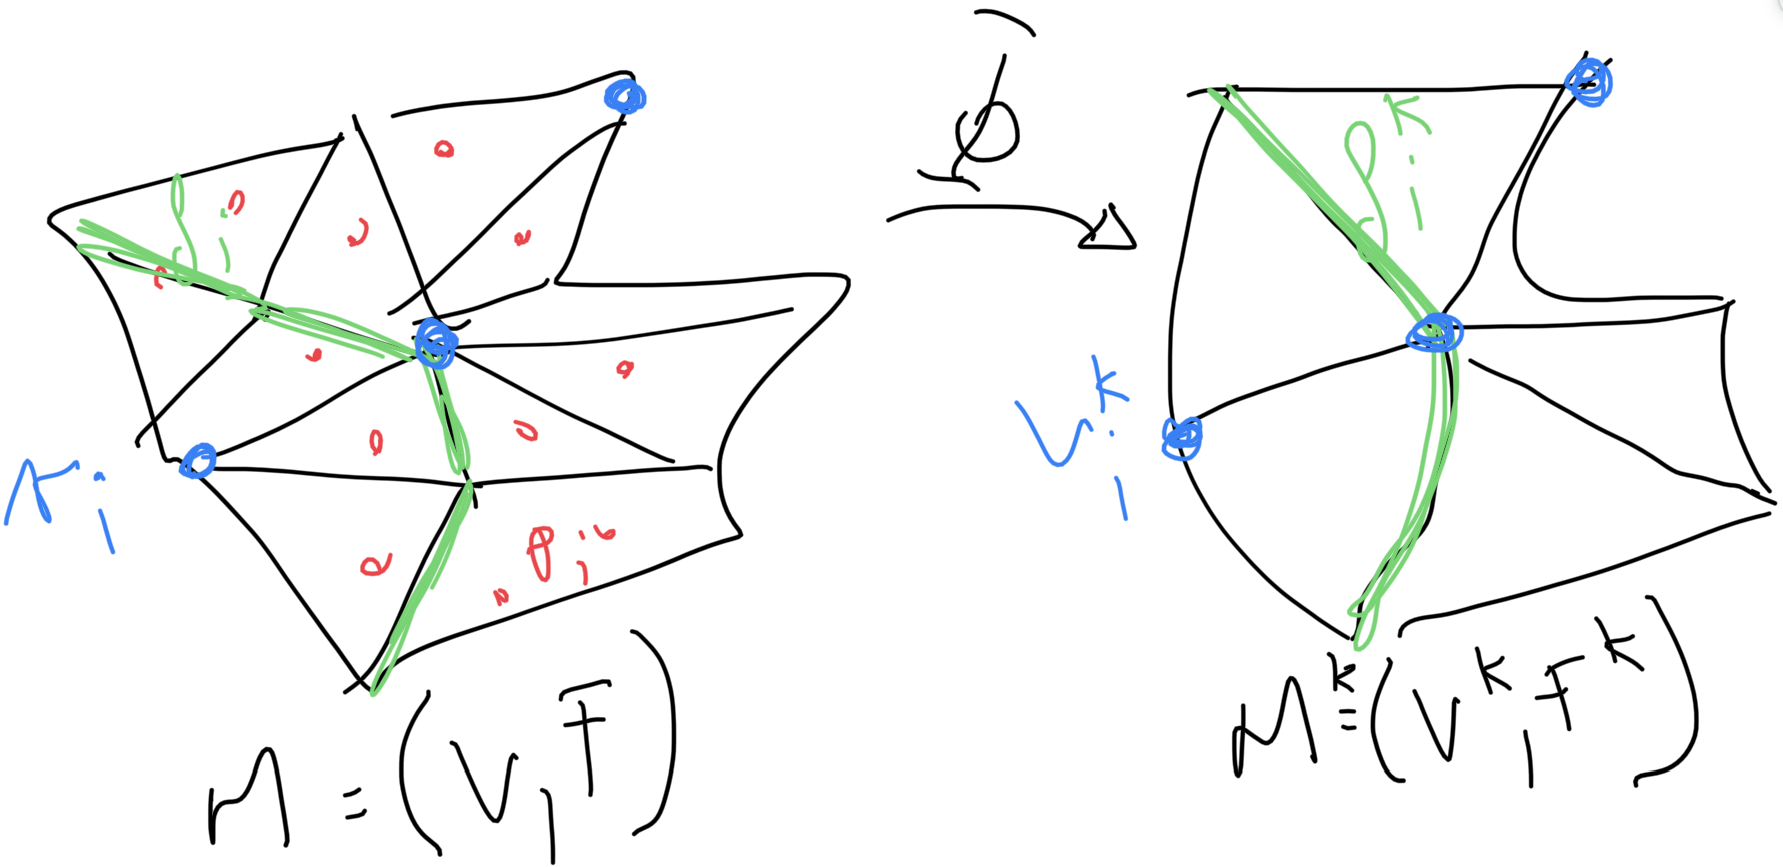
\includegraphics[width=\linewidth]{curve_meshing_in_shell_tex/figs/input-output}
    \caption{Input triangle mesh with features and output curved mesh with feature preserved equipped with bijective map $\phi^k$.}
    \label{bichon:fig:input-output}
\end{figure}

\paragraph{Input.}
The input of our algorithm is a manifold, watertight (enclosing a linear polyhedral volume), self-intersection free triangle mesh $\M=(V,F)$, and a set of points $p_i\in\P$ on the surface of $\M$ (Figure~\ref{bichon:fig:input-output} left). \DP{No parameters? Sizing, quality threshold, etc?} \ZJ{Sizing should be the coarsest possible, quality threshold is experimental on the particular implementaion rather than algorithm: } \DP{Mmm I think sizing should be exposed, it is useful for FEM.}
\ZJ{ok, sizing could be a parameter, but the current algorithm may not support that.} Optionally, our algorithm takes as input a set of feature edges $f_i\in\F$ and feature vertices $v_i\in\V$ such that no triangle in $F$ has more than one feature edge. (This property can be satisfied on any generic mesh by performing 1-to-3 refinement on every triangle with more than one feature edge).


\begin{figure}
    \centering
    \includegraphics[width=.6\linewidth]{curve_meshing_in_shell_tex/figs/nodes}\hfill
    \includegraphics[width=.37\linewidth]{curve_meshing_in_shell_tex/figs/gmapping}
    \caption{Nodes for different $k=1,2,3$ and example of geometric mapping $g$.\ZJ{illustration tip: different color/shape for vertex/edge/face/volume nodes}}
    \label{bichon:fig:high-order}
\end{figure}

\paragraph{Output.}
The output of our algorithm is a tetrahedral mesh $\M^k = (V^k,T^k)$ of order $k$. Formally, each tetrahedra $T\in T^k$ is defined through the order $k$ \emph{geometric mapping} from the reference tetrahedron $\hat T$
\[
g^T = \sum_{j=1}^n c_j^T L_j(\hat u,\hat v,\hat w),
\]
where $\hat u,\hat v,\hat w$ are the local barycentric coordinates of a point in $\hat T$, $c_j^T$ are the control points for a tetrahedron $T$, and $L_j$ are polynomial bases (typically Lagrange bases). Figure~\ref{bichon:fig:high-order} shows the position of the nodes $c_j$ on the reference element for $k=1,2,3$. We call the tetrahedralization of a curved mesh $\M^k$ \emph{positive} if $\det(J_{g^T }) > 0$ for every $T$. That is, we require that the geometric mapping $g$ is bijective for every tetrahedron. Note that for $k=1$, since $g$ is linear and affine, $J_{g^T }$ is constant and the positivity reduces to the common positive volume condition.


If the input has feature, the output curved mesh $\M^k$ will also have features edges $f_i^k\in\F^k$ and feature vertices $v_i^k\in\V^k$. To ensure that $\M^k$ closely approximates $\M$ we ensure that the distance from any point in $\P$ to $\partial\M^k$ (the surface of $\M^k$) is smaller than an user-controlled parameter $\varepsilon$.

Our algorithm guarantees that the tetrahedralization is positive and that $\M^k$ does not contain self-intersection. It also aims at coarsening $\M^k$ as much as possible while striving to obtain a  good geometric quality (controllable by the parameter \DP{XX}). 

To enable transfer of quantities between $\M$ and $\partial\M^k$ our algorithm produces a bijective map 
\[
\phi^k \colon \M \to \partial \M^k
\]
that preserve features by bijectively mapping $\F$ to $\F^k$ and $\V$ to $\V^k$. 

\paragraph{Overview.} Our algorithm starts by creating a mesh $\M^k$ that satisfies the following invariants:
\begin{enumerate}
    \item $\phi^k$ is bijective;
    \item $\phi^k$ bijectively maps $\F$ to $\F^k$ and $\V$ to $\V^k$;
    \item the distance between any $p\in\P$ and $\partial\M^k$ is less than $\varepsilon$;
    \item $\M^k$ is positive (i.e., every geometric map is bijective) \DP{why no symbol for geometric maps, also no definition of geometric map?}.
\end{enumerate}
It then performs local operation to improve $\M^k$ (i.e., coarsen it and improve its quality) while ensuring all the invariants are satisfied after each local modification. We use exact predicates for all invariants, ensuring correctness despite the use of floating point computations in our reference implementation of the algorithm. To achieve this goal our algorithm has two stages: (1) shell generation and (2) tetrahedral mesh generation.


\begin{figure}
    \centering
    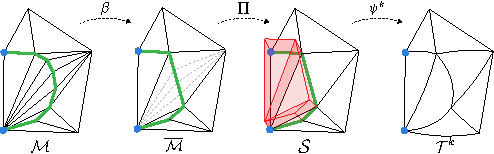
\includegraphics[width=\linewidth]{curve_meshing_in_shell_tex/figs/stage-1}
    \caption{Overview of the construction of the first stage of our pipeline}
    \label{bichon:fig:stage-1}
\end{figure}
\paragraph{Stage 1: Shell Construction.}
In the first stage (Section~\ref{sec:surface}) we extend the shell construction of \cite{jiang2020bijective} by preserving feature in $\F$ and $\V$; that is we construct a \emph{valid} shell $\PS$ with respect to the input surface $\M$ (i.e., $\M$ is a section $\PS$) that preserve features; to simplify the explanation we call $\PS$ a \emph{\ps{}} and call the prismatic projection $\Pi$. Together with the construction of $\PS$, we build an order $k$ \emph{prismatic shell} $\prS$ that defines a curved layer around $\M$ and a \emph{bijective} map $\xi^k$ between $\prS$ and $\PS$ (Figure~\ref{bichon:fig:stage-1}). Note that we do not require $\M$ to be a section of $\prS$.

To facilitate the second stage, we restrict the top and bottom surface of $\prS$ to be linear independently from the order of $\xi^k$. The output of this first stage is a high-order volumetric shell (linear on its boundary, curved on the interior), a feature preserving bijective mapping $\phi^k = \Pi \circ \xi^k$, and a trivial \emph{positive} tetrahedralization of $\prS$ with flat boundary. In other words, the tetrahedralization of $\prS$ satisfies all invariants.

\paragraph{Stage 2: Tetrahedral Mesh Generation.}
In the second stage (Section~\ref{sec:tets}) we use boundary-conforming tetrahedralization to connect the top and bottom surface of $\prS$ with a background tetrahedral mesh, thus generating a \emph{positive} order $k$ tetrahedralization $\M^k$ of a bounding box around the input, which we can further optimize with local operations to improve its quality. % Note that this pipeline  decouples the surface generation and feature preservation problem from the conforming volumetric tassellation, enabling us to tackle these two challenges independently.



\subsection{Feature-Preserving, Curved Shell Construction}\label{sec:surface}
To simplify the explanation, we first focus on the case where $k=1$ and $\varepsilon = \infty$, that is, we aim at generating a as-coarse-as-possible linear mesh and the feature preserving bijective mapping $\phi^1 = \Pi \circ \xi^1$. We then extend this construction to ensure a user-controlled distance bound $\varepsilon$ from the input (Section \ref{sec:distance}), and finally generalize to high-order geometric maps (Section \ref{sec:high-order}).

\begin{figure}
    \centering
    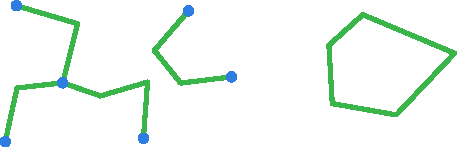
\includegraphics[width=0.5\linewidth]{curve_meshing_in_shell_tex/figs/feat-gr}
    \caption{The input edges feature (green) are grouped together in poly-lines and categorized in graph (left) and circles (right). For every graph we add the nodes (blue) to the set of feature vertices.}
    \label{bichon:fig:feat-gr}
\end{figure}

\paragraph{Feature Grouping.}
\DP{To discuss, consider moving in the input.}
The first step of our pipeline consists of grouping successive edges $f_i\in\F$ into poly-lines and identifying two categories: circle and graphs (Figure~\ref{bichon:fig:feat-gr}). For every graph, we identify its nodes and add them as feature vertices. In other words, we add to $\V$ all the end-points and junction of poly-lines.


% \begin{figure}
%     \centering
%     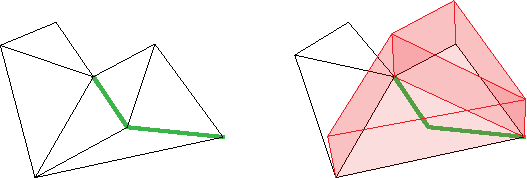
\includegraphics[width=\linewidth]{curve_meshing_in_shell_tex/figs/not-feat-pres}
%     \caption{Input feature is not preserved after traditional shell simplification.}
%     \label{bichon:fig:not-feat-pres}
% \end{figure}

% \paragraph{Limitation of the projection Operator of \cite{jiang2020bijective}.}
% \TS{change me}

\begin{figure}
    \centering
    \includegraphics[width=.5\linewidth]{curve_meshing_in_shell_tex/figs/zig}
    \caption{Illustration of a macro prism.}
    \label{bichon:fig:zig}
\end{figure}

\paragraph{Macro Projection Operator.} 
The shell construction introduced in \cite{jiang2020bijective} cannot preserve features or open boundaries. The authors \TS{us :D} suggested to freeze these vertices to ensure they are maintained in the projection. This comes with the disadvantage that the shell cannot be coarsened or improved next to features. To overcome this limitation we propose to ``group'' prism next to a feature into one big macro-prism.
% for instance, when performing an edge collapse on the feature  the new coarse edge (orange) will not map to the poly-line (green) anymore (Figure~\ref{bichon:fig:not-feat-pres}). To overcome this limitation we propose to change the \ps{} $\PS$ to guarantee that is contains the feature while building $\prS$ and the mapping $\xi^1$. 

Let $P$ a prism adjacent to a feature poly-line $f\in\mathcal{F}$ defined as a chain of $n$ oriented vertices $f_i, i=1,\dots,n$. The macro-prism $P$ is defined as the union of the $n-1$ \emph{sub-prisms} $P_i$ (Figure~\ref{bichon:fig:zig}) with middle surface $(v_1, f_i, f_{i+1})$. The macro projection operator for $P$ is simply defined as the union of the of the sub prismatic maps over each sub-prism $P_i$. We note that this definition does not ensure that the top and bottom surface of the macro-prism are flat.

% \begin{theorem}\label{th:bijective}
% The projection operator $\Pi$ defined as the \TS{union?} of projection operators (possibly radial) $\Pi_P$ is bijective if (1) the volume of every prism $\Pi_P$ and sub-prism $P_i$ is positive and (2) the top and bottom surface are intersection free.
% \end{theorem}
% \begin{proof}
% It trivially follows from other paper\TODO{check which theorem}.
% \end{proof}

To ensure the \ps{} with macro-prisms is valid we need ensure that $\Pi$ is bijective and that the normal condition holds for every prism and sub-prism; which is equivalent to ensure that for every prism (including sub-prsims) the shell is valid.
% As in~\cite{jiang2020bijective}, for every prism (including sub-prsims)  we check for positivity of the volume of the by ensuring that the tetrahedral decomposition has positive volume, use collision detection to check if the top and bottom are intersection free, and ensure that normal condition holds. This stage ensure that $\Pi$ satisfies the first two invariants.

We note that the initial shell in \cite{jiang2020bijective} is a valid feature preserving shell, as all feature poly-lines $f_i$ are composed by only two vertices. We extend the local operation to account for the poly-line: a collapse of a feature, requires to take the union of the poly-lines; while a split (or a smoothing) only requires splitting (or sliding a vertex) a poly-line (Appendix~\ref{app:local-ops}).


\begin{figure}
    \centering
    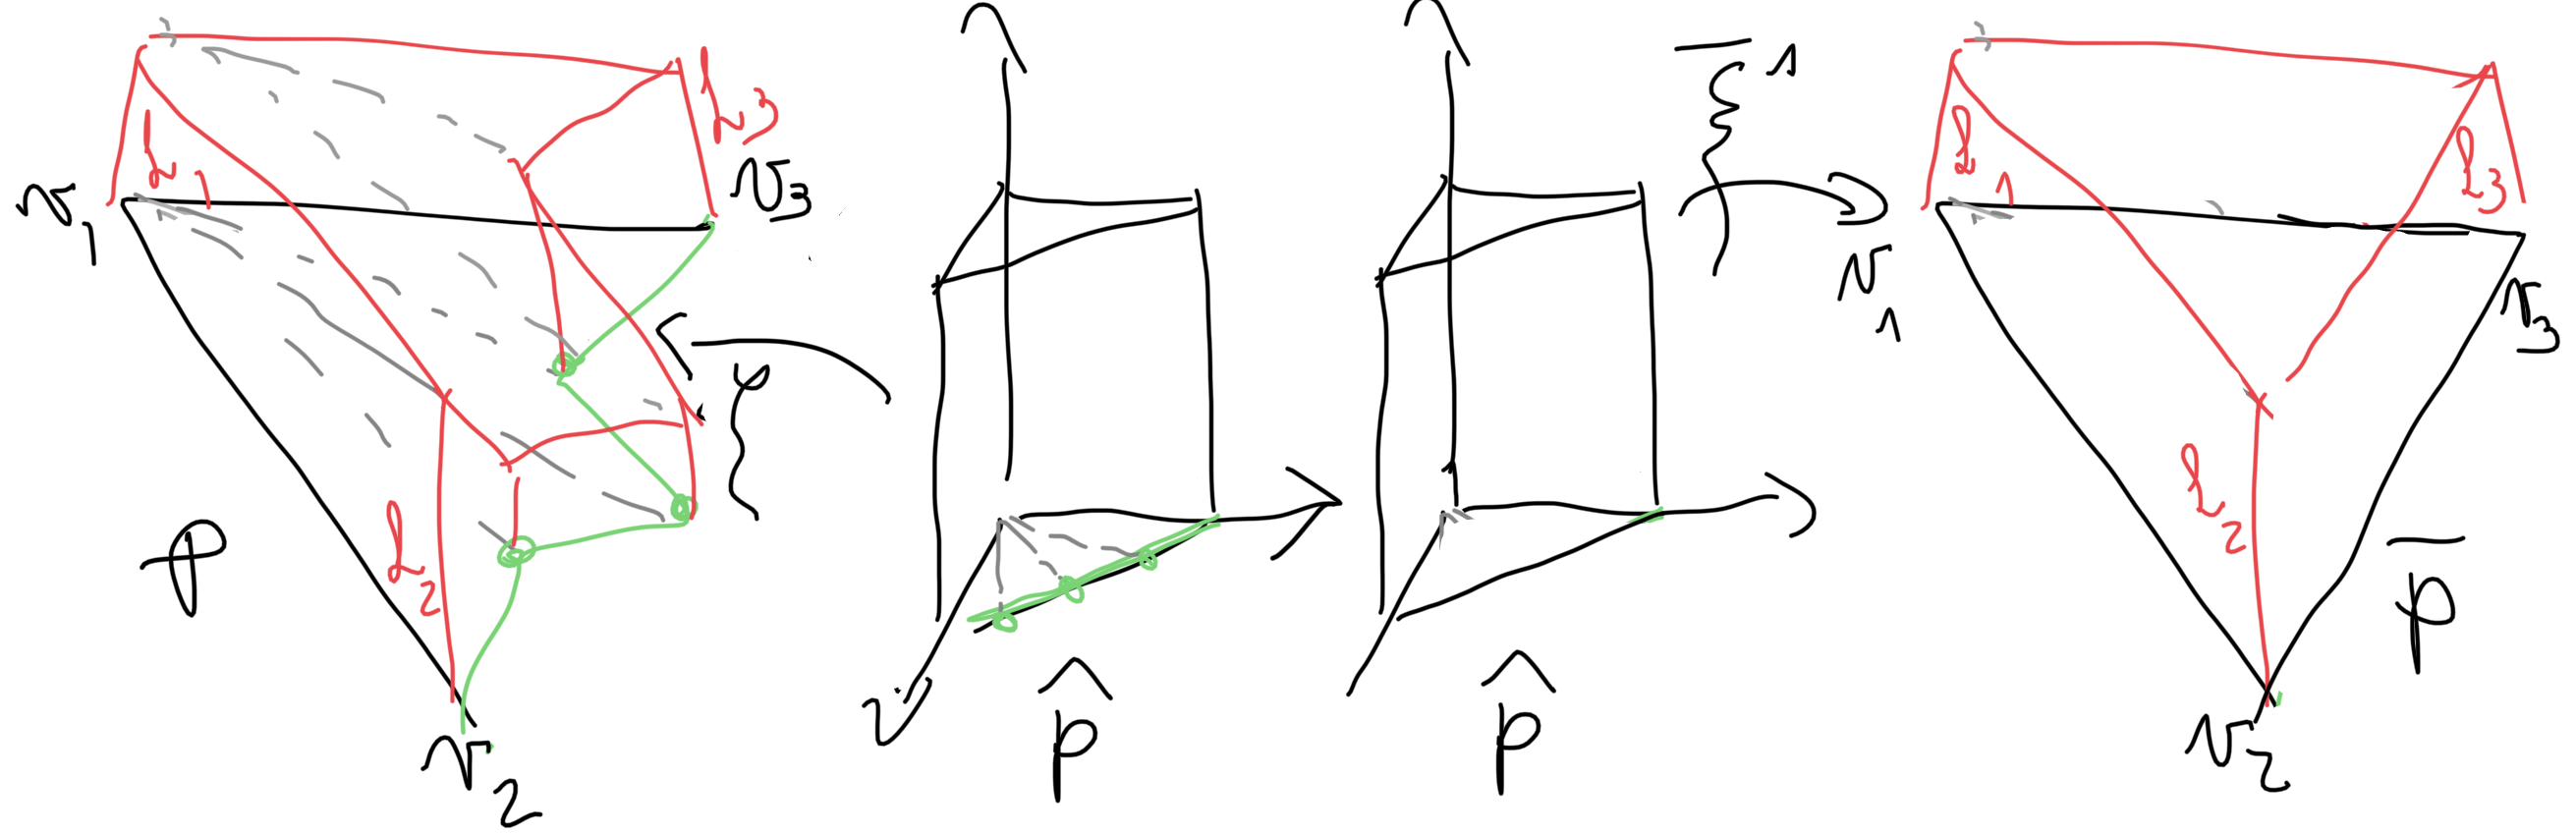
\includegraphics[width=\linewidth]{curve_meshing_in_shell_tex/figs/mappings}
    \caption{Example of mapping from $P$ to $\bar P$ passing through a reference prism $\hat P$.}
    \label{bichon:fig:ref-mapping}
\end{figure}


\paragraph{Coarse linear shell.} 
At this point we defined the feature preserving \ps{} $\PS$, however its middle surface is not a coarse mesh, but a ``fan'' of triangles.
To overcome this limitation, we construct a shell $\prS$ and the bijective map $\xi^1$ while optimizing for $\PS$. The shell $\prS$ is simply constructed by ``ignoring'' the poly-line vertices. Since $\phi^1 = \Pi \circ \xi^1$ and $\Pi$ satisfies the first two invariants, we only need to ensure that $\xi^1$ is bijective.

That is, for a prism $P\in\PS$ with mid-surface vertices $v_1, v_2, v_3$ and feature poly-line $f\in\mathcal{F}$, its corresponding prism $\bar P \in \prS$ is defined only by the three vertices $v_1, v_2, v_3$ and three pillars $h_i^T, h_i^B, i=1,2,3$.

To define the mapping $\xi^1 = \zeta\circ(\bar\xi^1)^{-1}$ we use two cross-paramterization maps from the reference prism $\hat P$: 
\[
% \text{(1) } 
\zeta \colon \hat P \to P \qquad
% \text{(2) } 
\bar\xi^1 \colon \hat P \to \bar P.
\]
The mapping from $\bar P$ is trivial as it is the tensor product between the base barycentric coordinates and $\bar P$ heights.

To define $\zeta$ we decompose the edge $(\hat v_2, \hat v_3)$ into $(\hat f_i, \hat f_{i+1})$ collinear segments whose length is proportional to $(f_i, f_{i+1})$. In other words we use the arc-length parameterization to map the polyline from $f$ to $\hat f$. Using this definition we then triangulate $\hat P$ in the same way as $P$ and map every sub-prism from $P$ to its corresponding one in $\hat P$ (Figure~\ref{bichon:fig:ref-mapping}).

The last part is to ensure that $\xi^1$ is bijective, which requires that both both $\zeta$ and $\bar\xi^1$ are bijective. The mapping $\zeta$ is bijective since $\Pi$ is, thus we only need to ensure that $\bar\xi^1$ has positive Jacobian which we check by representing $\det(J_{\bar\xi^1})$ using Berstein bases and exploit the convex-hull property of B\'ezier patches \cite{johnen2013geometrical}. Note that we do not require to check the normal condition since $\prS$ is not a valid shell with respect to $\M$.
To ensure global bijectivity of the \TS{union} of the mapping we only require that the boundary of the prisms $\bar P$ does not intersect which we explicitly check by collision detection. 

\paragraph{Results.} \DP{TODO}
Boundary coarsening + feature coarsening.
%%%%%%%%%%%%%%%%%%%%%%%%%%%%%%%%%%%%%%%%%%%%%%%%%%%%%%%%%%%%%%%%%%%%%%%%%%
%%%%%%%%%%%%%%%%%%%%%%%%%%%%%%%%%%%%%%%%%%%%%%%%%%%%%%%%%%%%%%%%%%%%%%%%%%

\subsubsection{Distance Bound}\label{sec:distance}

In the previous section we explained how to generate a feature preserving coarse linear shell. The output will be a coarse shell $\prS$ whose middle surface can be bijectively mapped to the input triangle mesh $\M$ and whose coarse feature edges are mapped to the input features. To ensure that the middle surface is both coarse and has a controlled distance from the points in $\P$, we interleave a distance check in the construction of $\bar\xi^1$ after each local operation. Formally, after every local operation we use the mapping $\phi^1$ to map every point $p_i\in\P$ to $\bar p_i = \phi^1(p_i)$ a point on the coarse middle surface of $\prS$ and, if $\|p_i-\bar p_i\| \geq \varepsilon$ we reject the operation. The initial shell is trivially a valid initialization as $\phi^1$ is identity and thus the distance is zero. Note that, $\bar p_i$ is not necessarily the closest point to $p_i$ on $\partial\M$, thus $\|p_i-\bar p_i\|$ is an upper bound on the actual pointwise distance.  \TS{normals?} \ZJ{Same procedure, still on my todo list.}


\paragraph{Results.} \DP{TODO}
single model, many different distance values.


\subsubsection{High-order}\label{sec:high-order}
In the previous section we explained how to generate a feature preserving distance bound coarse linear shell, that is an output that satisfies all invariants. The output will be a coarse shell $\prS$ with piecewise linear middle surface; to facilitate the coarsening of the middle surface we curve it, which accounts for changing the mapping $\xi^k = \zeta\circ (\bar\xi^k)^{-1}$ ($k > 1$), in particular the mapping $\bar\xi^k$. We note that, to decouple the following tetrahedral mesh generation and the curved shell generation, we ensure that $\bar\xi^k$ maps the top and bottom face of $\bar P$ to a linear triangle.

After each local operation, we generate samples $\hat s_i, i=1,\dots,m$ on the parametric base of the prism $\hat P$ and use $\Pi^{-1}\circ \zeta$ to map $s_i$ back to $\M$ and $\bar \xi^k$ to map them to $\partial\M$. Using the mapped point we solve
\[
\min_{c_i} \sum_{i=1}^m \|
(\Pi^{-1}\circ \zeta)(\hat s_i) - 
\bar \xi[c_i]^k(\hat s_i)
\|_2^2,
\]
where $c_i$ are the control points of $\bar\xi^k$. 
\TS{need more formal definitions?}.
We note that the control points of the top and bottom surface are fixed to ensure that $\bar\xi^k$ maintains the two surfaces as linear. As for the linear case we need to ensure that $\bar\xi^k$ is bijective which we check using the convex-hull property~\cite{johnen2013geometrical} and that the top and bottom surfaces are intersection free which is the same as in is linear since the top and bottom surfaces are flat.


\paragraph{Results.} \DP{TODO}


%%%%%%%%%%%%%%%%%%%%%%%%%%%%%%%%%%%%%%%%%%%%%%%%%%%%%%%%%%%%%%%%
%%%%%%%%%%%%%%%%%%%%%%%%%%%%%%%%%%%%%%%%%%%%%%%%%%%%%%%%%%%%%%%%
\subsection{Boundary Conforming Tetrahedral Meshing}\label{sec:tets}

\TODO{not done yet}
Then we need to fill in the space defined by bottom surfaces.
To this end, we require a linear tetrahedral meshing that respect the boundary precisely.
We deviate from the classical formulation
\cite{chew1989constrained,alexa2020conforming}\ZJ{Verify chew formulation} as follows: we do not want Steiner points on the boundary, but we can accept them in the interior.
To this end, we propose a simple but numerically robust algorithm to fill the interior. (Faster algorithm can be used if they succeed)
\begin{enumerate}
    \item Extrude a surface inside the domain, and connect with shell connectivity.
    \item in rational coordinates, perform robust binary spatial partitioning.
    \item split the generalized prisms without modify the surface.
    \item Smoothing and mesh operation until all the coordinates are representable in floating-point coordinates. \cite{hu2018tetrahedral}
\end{enumerate}

\paragraph{Results and comparison with CDT} \DP{TODO}


one example where CDT fails and we do not, robustness test on dataset, statistics on quality vs CDT on a subset where they both succeed.

\paragraph{Curved Tetrahedral Mesh Optimization}
smoothing: one vertex neighbor at a time (about 200 high order nodes).

mesh editing: split, collapse and swap.

